\begin{figure}[!tb]
    \centering
    \begin{subfigure}{0.45\textwidth}
        \centering
        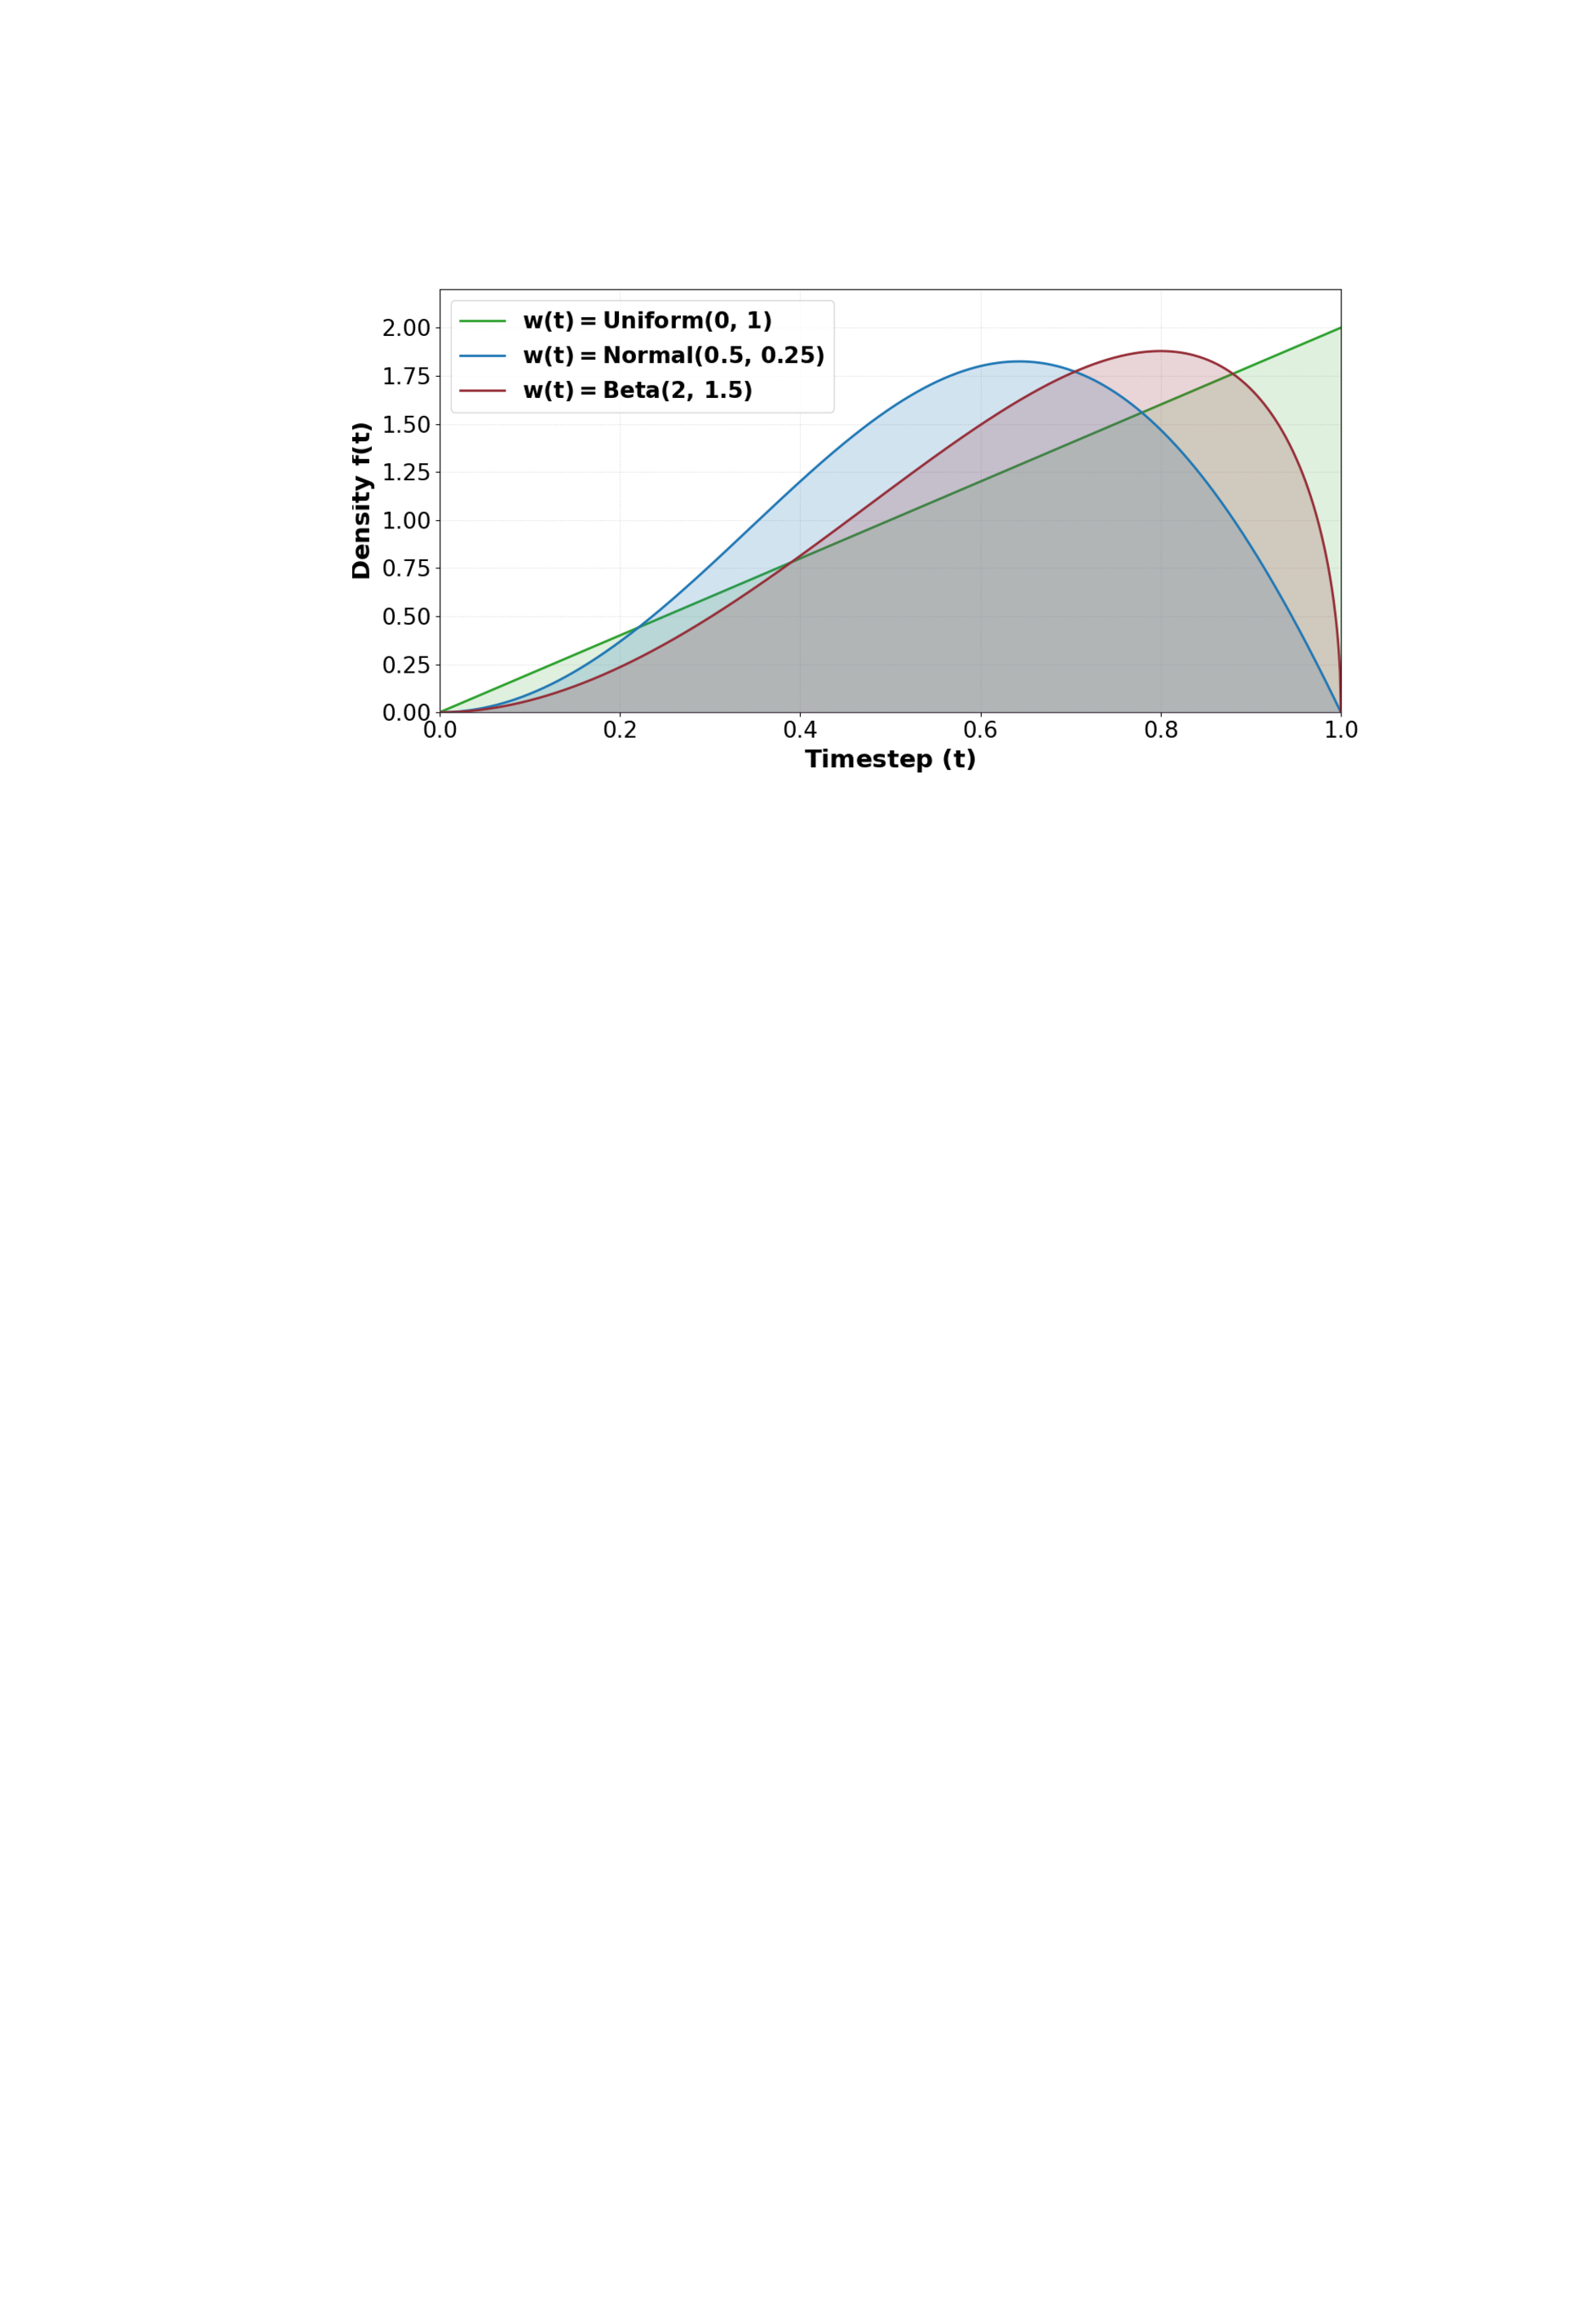
\includegraphics[width=\textwidth]{figures/src/time_sampler.pdf}
        \caption{Timestep density $f(t)=p(t)\cdot w(t)$, where $p(t)=2t$.}
        \label{fig:vis_distribution}
    \end{subfigure}
    \hfill
    \begin{subtable}{0.53\textwidth}
        \centering
\renewcommand{\arraystretch}{1.55}
        \resizebox{\linewidth}{!}{\begin{tabular}{l|cc|cc}
    \toprule
    \multirow{2}{*}{$\mathbf{w(t)}$} & \multicolumn{2}{c|}{\textbf{Bidirectional}} & \multicolumn{2}{c}{\textbf{Causal}} \\
    \cmidrule(lr){2-3} \cmidrule(lr){4-5}
    & \textbf{4 NFEs} & \textbf{32 NFEs} & \textbf{4 NFEs} & \textbf{32 NFEs} \\
    \midrule
    $\text{Uniform}(0, 1)$    & 83.46 & 83.75 & \textbf{83.58} & 83.91 \\
    $\text{Normal}(0.5, 0.25)$  & 83.40 & 83.79 & 83.54 & 83.93 \\
    \rowcolor{mitblue}$\text{Beta}(2, 1.5)$   & \textbf{83.48} & \textbf{83.96} & 83.54 & \textbf{83.96} \\
    \bottomrule
\end{tabular}}
        \caption{Quantitative ablation (Vbench overall score) of the loss weight function $w(t)$.}
        \label{tab:ablation_time_sampler}
    \end{subtable}
    \caption{\textbf{Ablation Study of Loss Weight Function $w(t)$}. Among the different weighting strategies, $w(t) = \text{Beta}(2, 1.5)$ demonstrates the best performance across both architectures.}
\label{fig:ablation_time_sampler}
\end{figure}